\subsection{Multi-Tenancy in \themis}
\label{sec:multi-tenancy}

Each \themis node runs as a single process that assumes that it has exclusive
access to its intermediate disks and that it will not experience
memory pressure from other processes that results in swapping as long as it
does not exceed its configured memory limit. Its memory and disk management
subsystems (described in detail in~\cite{themis} and~\cite{tritonsort}) rely on
these assumptions and are the key enablers of \themis' I/O-efficiency and high
performance. Hence, running multiple \themis processes on a single node would
result in degraded performance since the processes would interfere with one
another.

\begin{figure}
  \centering
  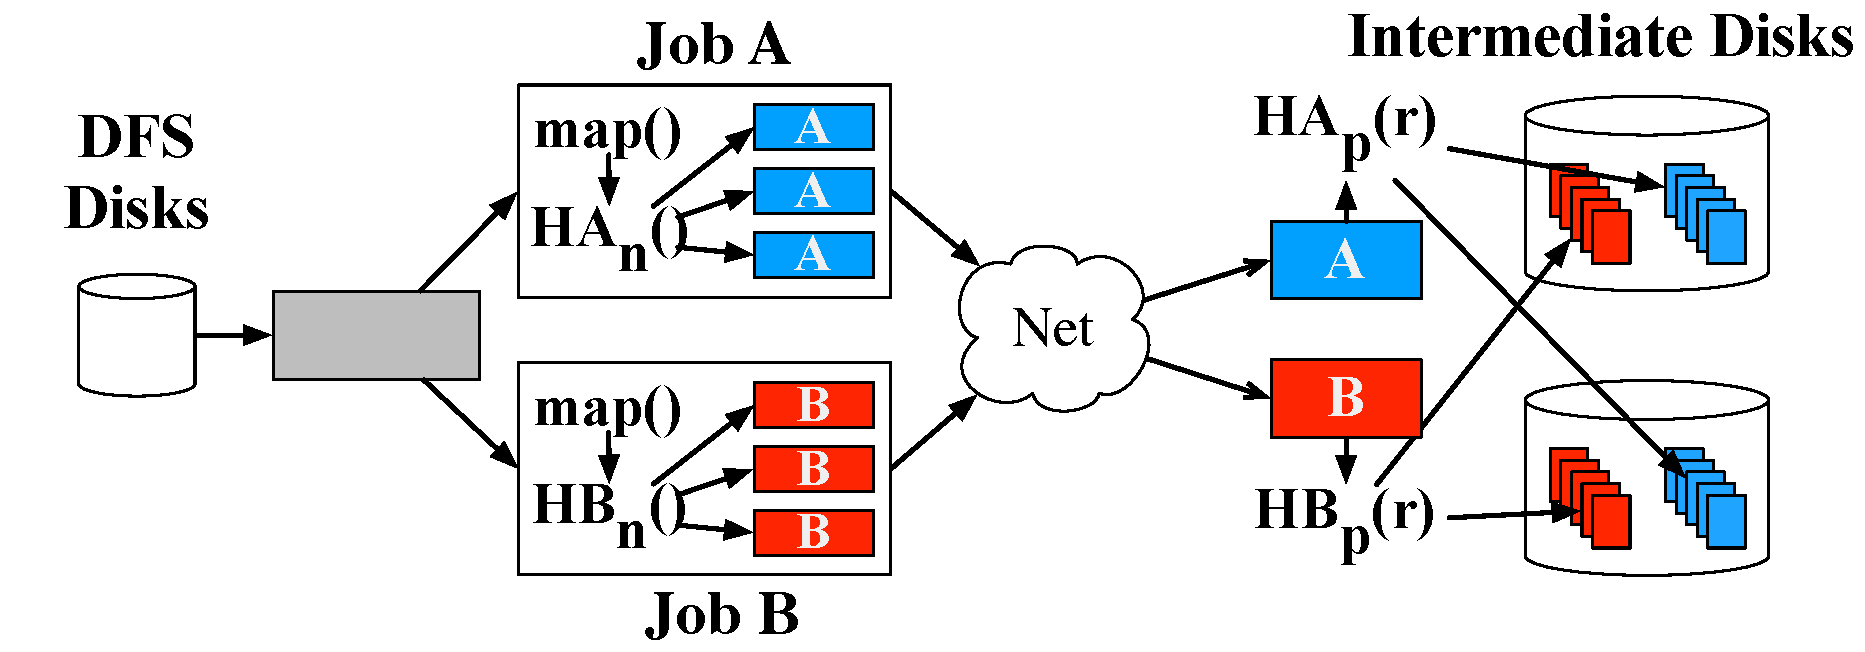
\includegraphics[width=\columnwidth]{fault_tolerance/figures/multi_tenancy}
  \caption{\label{fig:multi_tenancy} An overview of multi-tenancy in
\themis. Input records are mapped by both job A and job B's \map functions,
and intermediate records are routed based on each job's partition function independently.}
\end{figure}

To allow multiple jobs to run simultaneously in \themis with minimal
interference, we have modified \themis to support running multiple jobs
concurrently within a single process. To allow for this concurrent processing,
records read from disk are passed through each job's \map function one function
at a time, but intermediate records are transferred and written in
parallel. Buffers of intermediate records produced by a \map function are
tagged with the unique ID of that \map function's job before being sent to the
appropriate destination node. Once a buffer is received, this job ID is used to
determine to which set of intermediate partitions the buffer's records will be
written. This process is illustrated in Figure~\ref{fig:multi_tenancy}

A unique feature of our deployment prototype is that it does not co-schedule
\map and \reduce function computation. Instead, it organizes jobs into
\emph{batches}, and runs phases one and two for all jobs in a batch
simultaneously before processing the next batch. If phase zero needs to be run
to compute partition functions for any of these jobs, it is run on each job in
the batch individually before phase one starts.
